%% Template for a preprint Letter or Article for submission
%% to the journal Nature.
%% Written by Peter Czoschke, 26 February 2004
%%

\documentclass{nature}
%\documentclass[12pt]{article}

%% make sure you have the nature.cls and naturemag.bst files where
%% LaTeX can find them

\bibliographystyle{naturemag}

\usepackage{graphicx}
\usepackage{amssymb,amsfonts,amsmath}
\usepackage{subfigure}
\usepackage{stfloats}


%% OPTIONAL MACRO DEFINITIONS
\def\s{\sigma}
\newcommand{\be}[0]{\begin{equation}}
\newcommand{\ee}[0]{\end{equation}}
\newcommand{\lb}[0]{\left(}
\newcommand{\rb}[0]{\right)}


\title{Human-induced Arctic sea-ice loss and cold Eurasian winters}

%% Notice placement of commas and superscripts and use of &
%% in the author list


\author{Kelly E. McCusker,*$^{1,2}$ \& John C. Fyfe,$^{2}$ \& Michael Sigmond$^2$}

% NatGeo requirements:
% Title If possible, the title should give a sense of the main new finding, and should not exceed 90 characters, including spaces. Nature Geoscience titles do not contain technical terms or abbreviations unless absolutely necessary. We strongly discourage punctuation or active verbs.@@
% Letter 2,000 words no methods, 3 figures
% Article 3,000 words no methods, include section titles, 6 figures. No refs in abstract. ~500 words of Intro. 1-2 para of conclusions


\begin{document}

\maketitle

\begin{affiliations}
 \item School of Earth and Ocean Sciences, University of Victoria, Victoria, BC, V8P 5C2, Canada
 \item Canadian Centre for Climate Modelling and Analysis, Environment Canada, Victoria, BC V8W 2Y2, Canada
\end{affiliations}


\begin{abstract}
Arctic sea ice loss has been implicated in the recent trend toward unusually cold Eurasian winters \cite{liu12,mori14,kim14}. Whether the linkage follows from anthropogenic sea ice loss, however, remains an open question as the sea-ice loss combines anthropogenic response and internal (random) variability \cite{swart15,wettstein14} and because of confounding wintertime variability over the Eurasian continent \cite{deser12b,screen14a}. Here, we isolate the anthropogenic and random components of the linkage using a large ensemble of atmosphere-only model simulations with prescribed sea ice loss taken from simulations of the companion atmosphere-ocean-cryosphere model. We find no evidence of a sea-ice loss related decrease in Eurasian winter temperature. However, we do find long periods of winter Eurasian cooling linked to internally-generated circulation features over the Barents and Kara Seas regions of the Arctic. These results challenge the perception that Arctic sea ice loss was responsible for the recent prevalence of unusually cold Eurasian winters, showing instead that these winters were more likely the consequence of internal variability, with implications for our understanding of impacts and adaptation in human and natural high-northern latitude systems. %We find no evidence of a sea-ice loss related increase in the prevalence of cold Eurasian winters.
\end{abstract}

Average northern hemisphere winter (December-February; DJF) temperature has increased @@ $^\circ$C/decade since 1979. The majority of this warming is attributed to anthropogenic greenhouse gas emissions (@@cite) combined with positive feedbacks related to the loss of Arctic sea ice (@@cite). Epoch differences of surface air temperature (SAT) between 2002-12 and 1979-89 reveal warming upward of 2$^\circ$C over the polar cap, collocated with areas of sea ice loss (Figure \ref{fig:fig1}a). Contemporaneous cooling of greater than 1$^\circ$C over the Eurasian continent in winter is also evident. This feature is particularly striking when considered in the context of broad hemispheric warming. Eurasian winters show a greater prevalence of anomalous cold since the year 2000 in relation to the evolution of northern hemisphere temperature (Figure \ref{fig:fig1}b).   

%Figure \ref{fig:fig1}b shows the evolution of Eurasian winter SAT with hemispheric SAT removed to highlight the growing anomalous Eurasian cooling against hemispheric warming. Since 1979, eight of ten of the coldest Eurasian winters have occurred since the year 2000.

The recent tendency toward anomalously cold Eurasian winters has coincided with large reductions in autumn and winter sea ice area in the Barents and Kara Seas sector of the Arctic (along the eastern half of the Russian coastline); the nine lowest years have occurred since 2000 (Figure \ref{fig:fig1}c). Low sea ice concentration in the Barents-Kara Seas (BKS) has been linked to anomalously cold Eurasian SAT through a Rossby wave-train emanating out of the BKS region, incited by turbulent heat flux from an increased area of open water \cite{honda09,mori14,kim14,peings14}. However, while human influence on observed Arctic sea ice extent is clear \cite{min08}, interpretation of this Arctic sea ice--Eurasian SAT connection as an anthropogenic signal is limited by the strong imprint of internal variability on observed sea ice loss itself \cite{swart15}; internal variability may contribute approximately 50\% of the magnitude of the observed trend \cite{stroeve07,kay11}.

A clear anthropogenic signal in Arctic sea ice area changes during winter since 1979 is also evident in a comparison of a 50-member ensemble of simulations performed in the Canadian Earth System Model v2 (CanESM2) forced with all historical forcings (Historical; see Methods) versus 50 CanESM2 simulations forced with only natural forcings (HistoricalNat; Figure \ref{fig:fig2}). Whereas natural forcing yields nearly equal chances of sea-ice growth and sea-ice loss between (2002-12) and (1979-89), including anthropogenic forcing always yields sea-ice loss even in the face of large internal variability as indicated by the spread in the Historical distribution. Simulated Historical winter Arctic sea-ice area anomalies are consistent with satellite measurements of the Arctic sea-ice area anomaly from the National Snow and Ice Data Center (NSIDC). 


%Observations represent one potential reality out of many possibilities due to the random evolution of internally-generated variability super-imposed on a forced .%, although observations fall on the less-ice-loss side of the distribution.

%An observational estimate of sea ice loss from the National Snow and Ice Data Center (NSIDC) is consistent with simulated Arctic sea ice loss, however we note that the Historical large ensemble (LE) average overestimates observed winter sea ice loss.

%Observations represent one potential reality out of many, and thus are not expected to fall in any particular place on the Historical distribution, however the CanESM2 Historical ensemble compares favourably with the NSIDC observations.

Observations represent just one potential reality out of many due to the evolution of internally-generated (``random") variability superimposed on a human-induced (``forced") evolution. We isolate the effect of human-induced Arctic sea ice loss on the atmosphere by executing a large ensemble of Canadian atmosphere general circulation model (CanAM4) simulations in which prescribed past (1979-89) and present-day (2002-12) boundary conditions are taken from an average of five CanESM2 Historical simulations (Figure \ref{fig:fig2} and Supplementary Figure 1; also see Methods). The average boundary conditions represent an estimate of the human-induced component by averaging out internal variability. 

A set of five 120-year AGCM simulations, differing only in initial conditions, is executed with annually-repeating, monthly sea-ice concentration (SIC), sea-ice thickness (SIT), and sea surface temperature (SST) for ``past" boundary conditions and for ``present-day" boundary conditions in which the only changes are Arctic SIC, SIT, and SST (where SIC $<$ 15\% in the present day but not the past). The anomalies between these ``Average SIC forcing" past and present-day simulations estimate the isolated response of the atmosphere to human-induced sea ice loss. We similarly execute five pairs of 120-year AGCM simulations with boundary conditions taken from the individual CanESM2 Historical simulations (``Individual SIC forcing" ensemble) to represent the response to varying boundary conditions that incorporate internal variability. Thus in total, each ensemble consists of 600 years of (present - past) anomalies. In addition, we execute a pair of 120-year simulations with past and present-day NSIDC boundary conditions (Supplementary Figure 1).

We first present the responses of regionally-averaged winter SAT from all simulations as ``uncertainty cascades" \cite{wilby10,swart15}, where uncertainty is based on the number of simulation years averaged (Figure \ref{fig:fig3}). This presentation demonstrates the powerful influence of internal variability. A reduction in SIC reveals newly open seawater that provides a source of heat to the atmosphere. Thus, the local effect of human-induced sea ice loss, averaged across the Average SIC forcing ensemble (600-year average), is a warming over the polar cap (averaged north of 60$^\circ$N) of just over 1$^\circ$C in winter (bottom of Figure \ref{fig:fig3}a). When considering instead the 120-year averaged SAT responses to Average SIC forcing, a spread in responses is evident that ranges from $~$0.9$^\circ$C to 1.3$^\circ$C. The spread of 60-year averages is larger still. 

This spread is noteworthy because, given the identical boundary conditions for each 120-year and 60-year average, the range of anomalies must be due solely to internal variability. Furthermore, the range of 120-year average SAT responses in the Individual SIC forcing ensemble (top of Figure \ref{fig:fig3}a) is comparable to that of the Average SIC forcing ensemble, indicating that even local sensitivity of SAT to varied sea ice loss conditions is overpowered by internal variability in winter.    % @@ supplementary to show it is not the case in SON?

%two reasons: i. because the boundary conditions for each 120-year and 60-year average are identical, the driver of the differences must be solely internal variability, and ii. each anomaly presented (600-year, 120-year, and 60-year average) is statistically significant at the 90\% level. The implication is that  one could be mislead as to the true response if a simulation was stopped after just 60-years, or even 100, as has been common practice (@@). 
%previous findings indicate that 60 years is sufficient to determine a robust, local SAT response to sea-ice loss (e.g. Ref. \cite{screen14a}), which these results do not support. Furthermore, the range of 120-year average SAT responses in the Individual SIC forcing ensemble is comparable to that of the Average SIC forcing ensemble, indicating that sensitivity of SAT to varied sea ice loss conditions is overpowered by internal variability, even locally, in winter. 
%Furthermore, each anomaly presented (600-year, 120-year, and 60-year average) is statistically significant at the 90\% level, which would lead one to believe
%--- for example, the 60-year average of the present day polar cap SAT is significantly different from the past polar cap SAT. Thus, 

Moving farther afield, the SAT response over Eurasia is not statistically different from zero in either the Individual or Average SIC forcing ensemble averages, indicating that the robust response of Eurasian winter temperature to human-induced Arctic sea-ice loss is not cooling, but rather no signal (Figure \ref{fig:fig3}b). Nevertheless, some 120-year and 60-year average anomalies show statistical significance, most notably the 60-year average cooling associated with NSIDC SIC forcing that is not robust to the 120-year average. This point is important to recognize because many studies understandably utilize 60- to 100-year integrations to draw conclusions that may prove inaccurate given larger ensemble sizes.

Arctic sea ice loss can yield either warmer or cooler Eurasian SAT in winter, even with a large ensemble size of 120-years each, and even with identical boundary forcing (Figure \ref{fig:fig3}b). To understand this further, we examine the spatial pattern of circulation associated with the two ``extreme" cases of cold and warm SAT anomalies in the Average SIC forcing ensemble (Figure \ref{fig:fig4}). It is immediately apparent that the patterns of geopotential height at 500 hPa (Z500) are quite different from one another, and in some locations such as over the BKS, nearly opposite. The cooling case (Figure \ref{fig:fig4}a) shows a zonally-symmetric increase in Z500 to the north and a weak decrease over central Eurasia. This pattern is conducive for advection of polar air to the south and west along Z500 contours. In contrast, the warming case (Figure \ref{fig:fig4}b) exhibits an azonal pattern with a decrease in Z500 over the BKS region and increases over the southern continent and the northeast. This pattern favours warm-moist air advection from the south and west.

The relationship between the winter circulation, in particular over the Barents-Kara Seas, and Eurasian SAT is genuine and exists across 120-year average anomalies (Figure \ref{fig:fig5}). As Z500 anomalies over the Barents-Kara Seas increase, Eurasian SAT anomalies decrease, with a regression slope of -0.25$^\circ$C/10 m and a p-value of 0.002. This same relationship holds interannually within each individual simulation, with comparable slopes (@@) and significance (p<0.001). Thus, the physical mechanisms that lead to the Eurasian cooling case are consistent with existing work that implicates high geopotential heights over the Barents-Kara Seas region (cite@@). What is notable here, however, is that there is no indication that changes in sea-ice concentration are the fundamental origin of Eurasian SAT anomalies, because sea-ice concentration is prescribed in our simulations. 

% FOR Z500 vs Eurasian SAT
% -------- LENat slope, rval, pval: -0.0191453043517 -0.517080959729 0.000120620535074
% -------- LE slope, rval, pval: -0.0165286796574 -0.413836962376 0.00281317881451
% -------- SIMS slope, rval, pval: -0.0248522162816 -0.846875216236 0.00199086631714
% % FOR Z500 vs Eurasian SAT - NH SAT
% -------- LENat slope, rval, pval: -0.0197128206884 -0.59198196108 5.95247762651e-06
% -------- LE slope, rval, pval: -0.0171532999171 -0.483943293482 0.000369911726737
% -------- SIMS slope, rval, pval: -0.0230542520751 -0.839763760963 0.00236577158697


%In further support of this, we find no relationship between 120-year average BKS surface fluxes (turbulent or net flux) and Eurasian SAT, or BKS SAT and Eurasian SAT (not shown/supp?). This finding is consistent with \cite{woollings14} who found no relationship between BKS temperature and Eurasian blocking in CMIP5 models. Furthermore, we find no change in the frequency distributions of yearly Nov-Dec averaged Eurasian SATs between the simulations with past sea-ice boundary forcing versus present-day sea-ice boundary forcing (not show/supp?).

We have seen that neither human-induced sea-ice loss, nor observed sea-ice loss consistently causes Eurasian cooling in our simulations. Rather internal variability, even with a sample of 120 years, is the dominant effect. What, then, is the cause of Eurasian winter cooling in the observational record? Others have suggested changes in the North Atlantic SST \cite{sato14}, or increased blocking due to the phase of the Atlantic Multidecadal Oscillation and North American Oscillation \cite{peings14b}, both manifestations of internal variability in the climate system. Indeed, we find that the relationship between observed geopotential height over the Barents-Kara Seas and Eurasian SAT in winter are consistent with internal variability within the CanESM2 Historical Large Ensemble, when the northern hemisphere warm bias in CanESM2 is taken into account (Supplementary Figure \ref{fig:supp2b}). We conclude that while observed winter cooling over Eurasia may be exceptional against the sway of global warming, it is not outside the purview of internal variability.

%It may be driven initially by changes in North Atlantic SST, triggering planetary waves that lead to both BKS sea-ice loss and Eurasian cooling \cite{sato14}, or due to the phase of the Atlantic Multidecadal Oscillation and North American Oscillation increasing blocking episodes conducive to causing continental cooling \cite{peings14}. Either way, 

%LE: obs consistent with LE and explained by internal variability in Z500 (@@need to calc BKS sea ice though...)

% DJF BKS SIC vs DJF Eurasian SAT
%-------- LE slope, rval, pval: -0.0074382420652 -0.0346488346007 0.811199353265
%-------- LENat slope, rval, pval: -0.000227580762807 -0.000827438892856 0.995449778436
% SON BKS SIC vs DJF Eurasian SAT
%-------- LE slope, rval, pval: -0.0494854037864 -0.165053395902 0.252018009728
%-------- LENat slope, rval, pval: -0.0448787415459 -0.205436237571 0.152364693465
% @@ Note this relationship is opposite (more sea ice loss = warmer Eurasia!)

% DJF BKS SIC vs DJF BKS Z500  !!!
%-------- LE slope, rval, pval: -1.52694237681 -0.28408601672 0.0455664758446
%-------- LENat slope, rval, pval: -2.47825524983 -0.333618515181 0.0179016352366
% @@ More ice loss = higher heights! hmm



%The relationship is furthermore present in the CanESM2 Historical Large Ensemble, in which all components of the model are active, all historical forcings are included, and hence many realizations of sea-ice loss are produced (Supplementary Figure \ref{fig:supp2}).


%FROM PREV VERSION Here, however, SST changes in the North Atlantic are held fixed and cannot be implicated as the root cause. We conclude that while the simulated early winter relationship between circulation over the BKS and Eurasian SAT is robust and consistent with expectations of temperature advection, it does not favour one sign or another when forced with Arctic sea-ice loss. Instead, the circulation response to human-induced sea ice loss and the average (human-induced) circulation response to variable sea-ice loss, which together we refer to as the robust response, is a more pan-Arctic increase in geopotential heights in ND that are not localized or particularly strong over the sensitive BKS region (supp fig?). 

%We find that the observed Z500 anomaly over the Barents-Kara Seas and the cold Eurasian winter anomaly is within the 5-95\% confidence range of the CanESM2 Historical Large Ensemble, when the warm-bias in northern hemisphere SAT is taken into account (Supplementary Figure \ref{fig:supp2b}).


%@@concluding remarks should include: something about how if sea-ice loss does nudge Eurasian SAT in one way or another, the signal would be much too small in reality to distinguish from natural variability anyway.

% while the Individual SIC forcing ensemble mean polar cap SAT response is nearly identical to that of the Average SIC forcing, 
 

%The response of SAT over the polar cap (averaged north of 60$^\circ$N), where it is local to the sea ice loss, 

%Focusing on winter, we contrast the local response of SAT over the polar cap (Figure \ref{fig:fig3}a) with the remote response of Eurasian SAT (Figure \ref{fig:fig3}b)

%We first examine the response of SAT over the polar cap (averaged north of 60$^\circ$N) where it is local to the sea ice loss. Newly open seawaters provide a source of heat to the atmosphere, causing it to warm --- the Average SIC forcing ensemble mean, indicative of the response to human-induced sea ice loss, is a warming over the polar cap in winter (Figure \ref{fig:fig3}a). 

%The response of SAT in winter over the polar cap (averaged north of 60$^\circ$N) to human-induced sea ice loss is warming of just over 1$^\circ$C, indicated by the Average SIC forcing ensemble mean in Figure \ref{fig:fig3}a. 

%We show the response of regionally averaged SAT as an ``uncertainty cascade" \cite{wilby10,swart15} where uncertainty is based on number of years averaged. This presentation demonstrates the powerful and sometimes misleading effect of internal variability.

 %as well as demonstrate the powerful and sometimes misleading effect of internal variability 

%by prescribing to an atmosphere general circulation model (AGCM) sea-ice concentration (SIC), sea-ice thickness (SIT), and sea-surface temperature (SST) boundary conditions that are an ensemble average of five historical simulations from a fully-coupled global climate model (Figure \ref{fig:fig2}; also see Methods). The average boundary conditions represent an estimate of the human-induced component of the boundary condition by averaging out internal variability. Pairs of simulations are executed with the CanESM2's associated Canadian AGCM (CanAM4) in which past (1979-89) and present-day (2002-12) Arctic sea-ice conditions from the five CanESM2 Historical ensemble members that are included as part of CMIP5 (Figure \ref{fig:fig2}) are prescribed as boundary conditions (see Methods). 

%While the number of realizations averaged is small, it is 



%Interpretation of this connection as an anthropogenic signal, however, is limited by the strong imprint of internal variability on observed sea ice loss \cite{swart15}, which may contribute approximately 50\% of the magnitude of the observed trend \cite{stroeve07,kay11}.

%Human influence on observed Arctic sea ice extent since the early 1990's is clear \cite{min08}

%However, the magnitude, timing, and structural details of the Eurasian cooling differ between these findings and do not fully explain observed Eurasian cooling. 

%, and a robust connection remains elusive. Furthermore, a connection between % implying that a robust linkage between Arctic sea ice loss and Eurasian SAT is 

%Interpretation of the connection between observed Arctic sea ice loss and cold Eurasian SAT is further complicated by the imprint of internal variability on the sea ice loss itself \cite{swart15}, which may contribute approximately 50\% to the magnitude of the observed trend \cite{stroeve07,kay11}. %Thus, much of the 'forcing' in earlier work, the observed sea ice change, is itself due to internal variability. A critical question remains: Has human-induced sea ice loss caused colder Eurasian winter temperatures? 



\begin{methods}
\textbf{Observations} \\
blah blah blah
\\
\textbf{Model simulations}\\
blah
\end{methods}

\begin{figure}%[htbp] % the star afterwards makes it a one column fig in a 2-col document
\centering
\noindent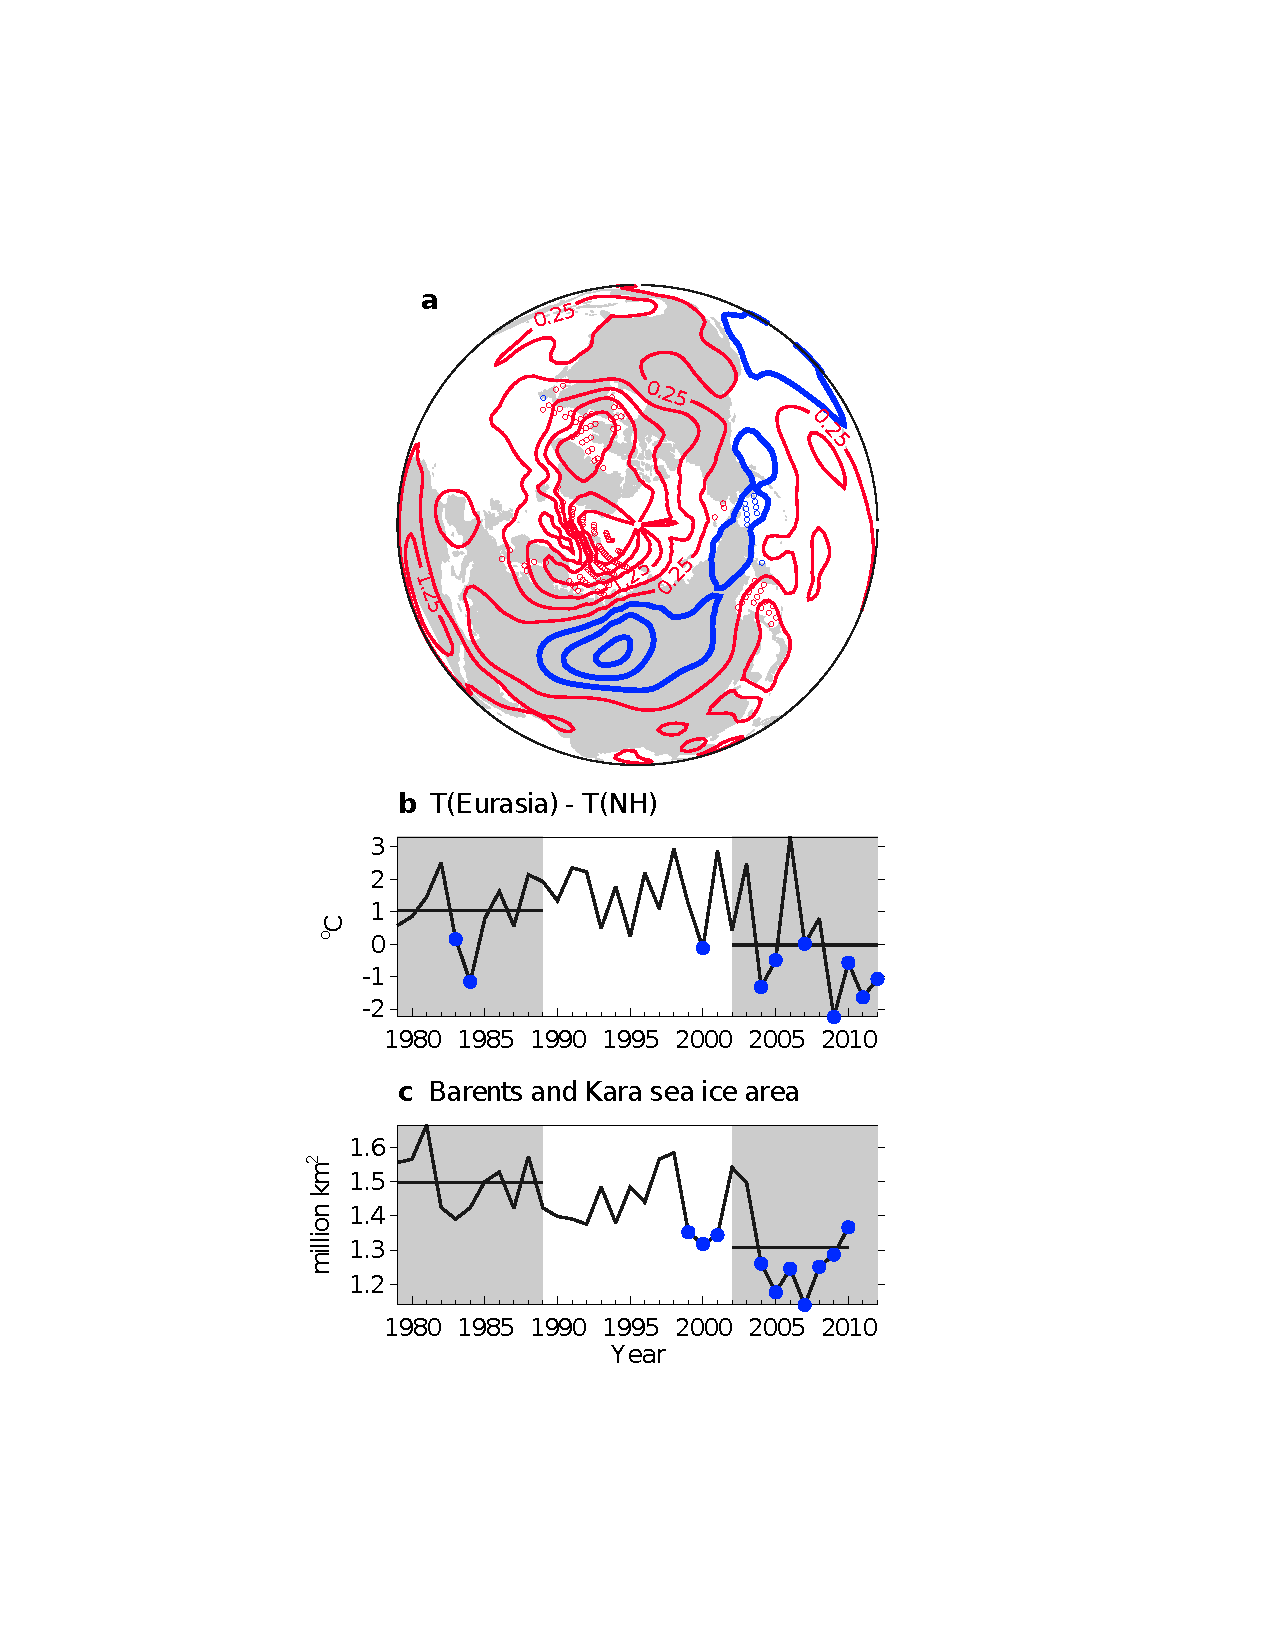
\includegraphics[width=19pc]{Figure1.pdf}
\caption{\textbf{Observed surface air temperature and sea ice concentration.} a.) Map of Gistemp winter surface air temperature anomalies as (2002-12) minus (1979-89) in contours. Contour interval is 0.5$^\circ$C with zero contour omitted. Open circle markers indicate regions of sea ice loss (red) and gain (blue) that are greater than 40\% in absolute terms. b.) Time series of Eurasian-averaged (35$^\circ$N - 60$^\circ$N, 40$^\circ$E - 120$^\circ$E) winter SAT with hemispheric (NH) winter temperature removed. Blue markers indicate the 10 most negative anomalies. c.) Time series of Barents-Kara Seas region (65$^\circ$N - 80$^\circ$N, 27$^\circ$E - 96$^\circ$E) winter sea ice area. Blue markers indicate the 10 lowest concentrations.
}
\label{fig:fig1} 
\end{figure}

\begin{figure}%[htbp] % the star afterwards makes it a one column fig in a 2-col document
\centering
\noindent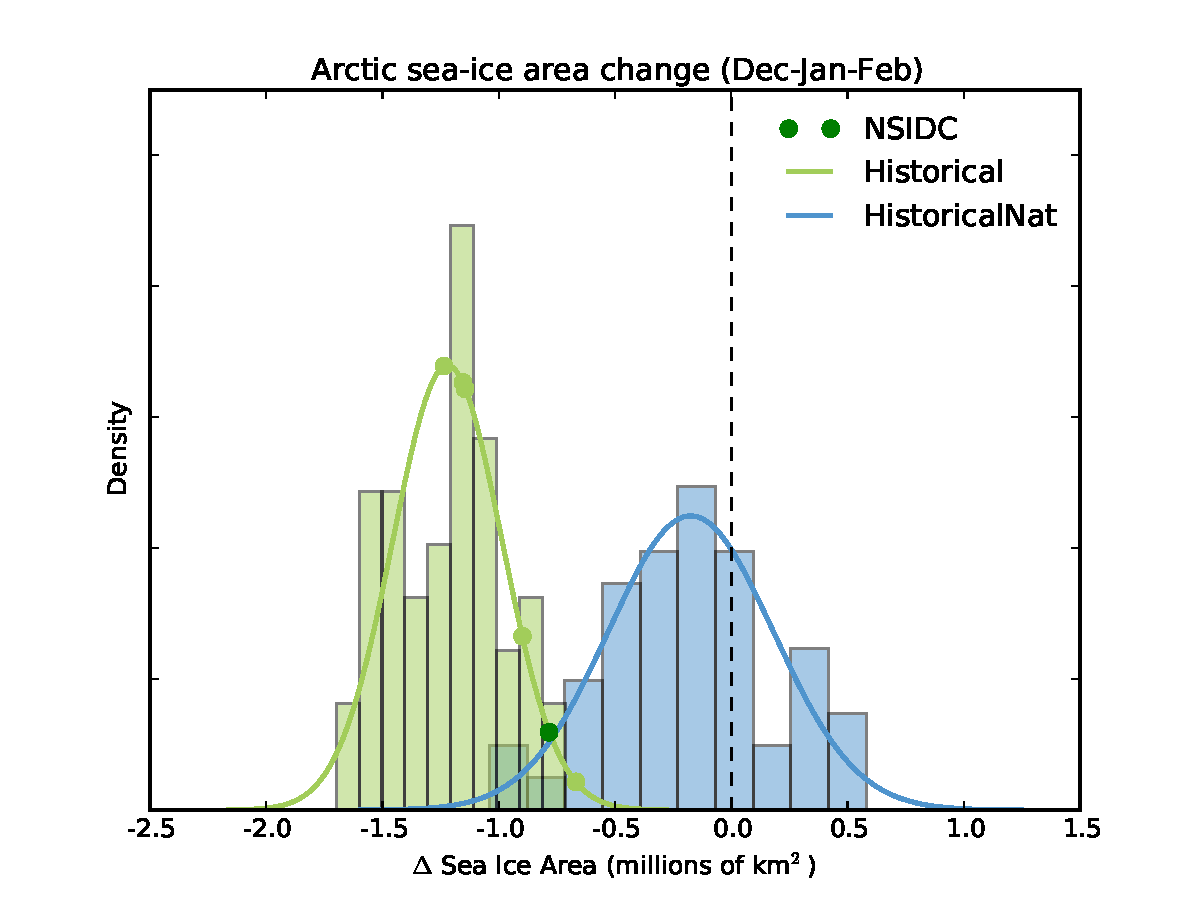
\includegraphics[width=25pc]{Figure2.pdf}
\caption{\textbf{CanESM2 large ensemble change in winter sea ice area.} Histograms and histogram fits of winter averaged Arctic sea-ice area changes from the period 1979-89 to 2002-12 in the CanESM2 Historical (light green) and HistoricalNat (blue) large ensembles (50 members each). Light green markers indicate the original five Historical simulations, published as part of CMIP5 and seeds for the Historical LE, and also prescribed as boundary conditions to our ’Individual SIC forcings’ AGCM simulations. The dark green marker shows Arctic sea-ice change from the NSIDC bootstrap observational dataset. Filled markers indicate the present day period (2002-12) is significantly different from the past (1979-89) at the 90\% level using the Student’s T test of difference between two means. 
}
\label{fig:fig2} 
\end{figure}

\begin{figure}%[htbp] % the star afterwards makes it a one column fig in a 2-col document
\centering
\noindent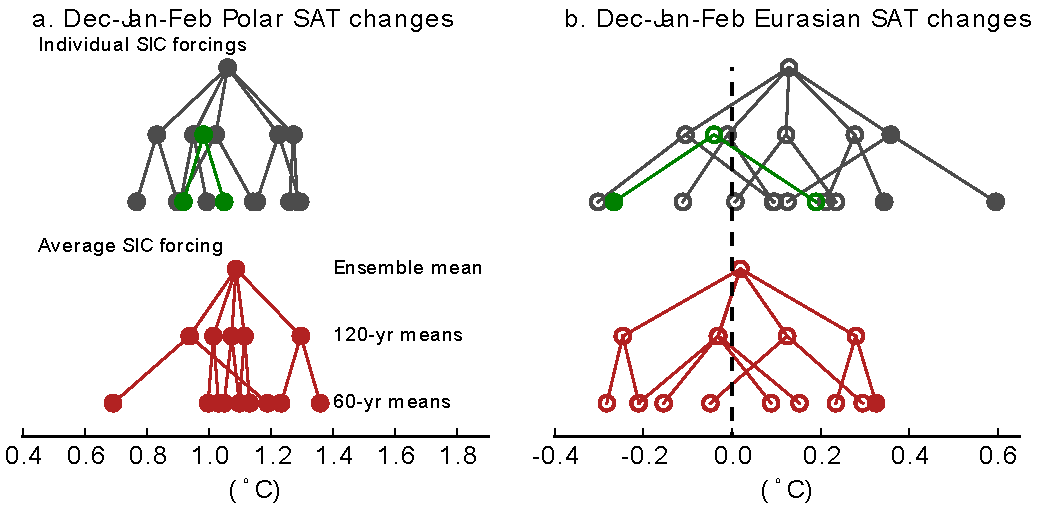
\includegraphics[width=35pc]{Figure3.pdf}
\caption{\textbf{Simulated polar cap and Eurasian temperature response uncertainty cascades.} Regional winter response of SAT to Individual SIC forcings (black) and Average SIC forcing (red) shown as uncertainty cascades of the a.) polar cap anomalies (averaged poleward of 60$^\circ$N) and b.) Eurasian anomalies (averaged within 35$^\circ$N - 60$^\circ$N, 40$^\circ$E - 120$^\circ$E). Each cascade consists of the ensemble average of five 120-year ensemble members (top level), individual 120-year ensemble member averages (middle level), and ensemble members sub-sampled into two 60-year segment averages (bottom level). Filled circles indicate significance at the 90\% level using the Student’s T test of difference between two means. 
}
\label{fig:fig3} 
\end{figure}

\begin{figure}%[htbp] % the star afterwards makes it a one column fig in a 2-col document
\centering
\noindent\includegraphics[width=39pc]{Figure4_orSuppFig2.pdf}
\caption{\textbf{Winter surface air temperature and geopotential height responses.} Winter average SAT change ($^\circ$C) with geopotential heights at 500 hPa in contours (contour interval = 3m).
}
\label{fig:fig4} 
\end{figure}

\begin{figure}%[htbp] % the star afterwards makes it a one column fig in a 2-col document
\centering
\noindent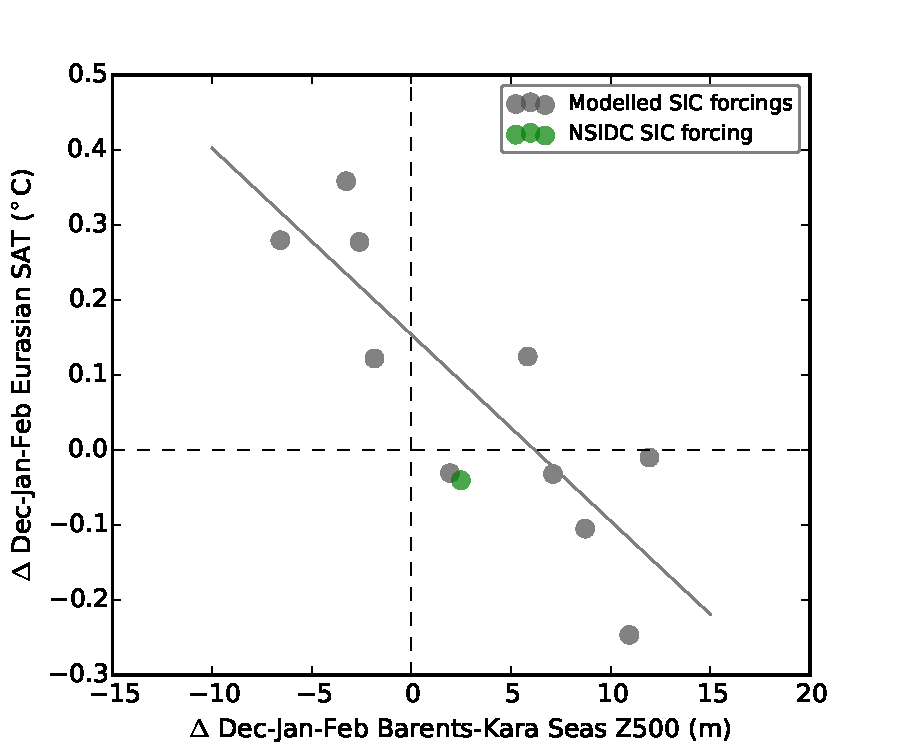
\includegraphics[width=25pc]{Figure5.pdf}
\caption{\textbf{Winter Eurasian surface air temperature versus Barents-Kara geopotential height.} Winter averaged Eurasian SAT ($^\circ$C) versus geopotential height at 500 hPa over the Barents-Kara Seas region (65$^\circ$N - 80$^\circ$N, 27$^\circ$E - 96$^\circ$E). Grey circles indicate 120-year average anomalies for each member of the Individual and Average SIC forcing ensembles, shown together because the distributions are statistically indistinguishable from one another (mean and variance of BKS Z500 and Eurasian SAT between the two ensembles are not different). The dark green marker indicates the 120-year average anomaly from the NSIDC SIC forcing simulation pair. The regression line ($r^2$ = 0.72, $p$ = 0.002) does not include the NSIDC SIC forcing simulation average.
}
\label{fig:fig5} 
\end{figure}

\begin{figure}%[htbp] % the star afterwards makes it a one column fig in a 2-col document
\centering
\noindent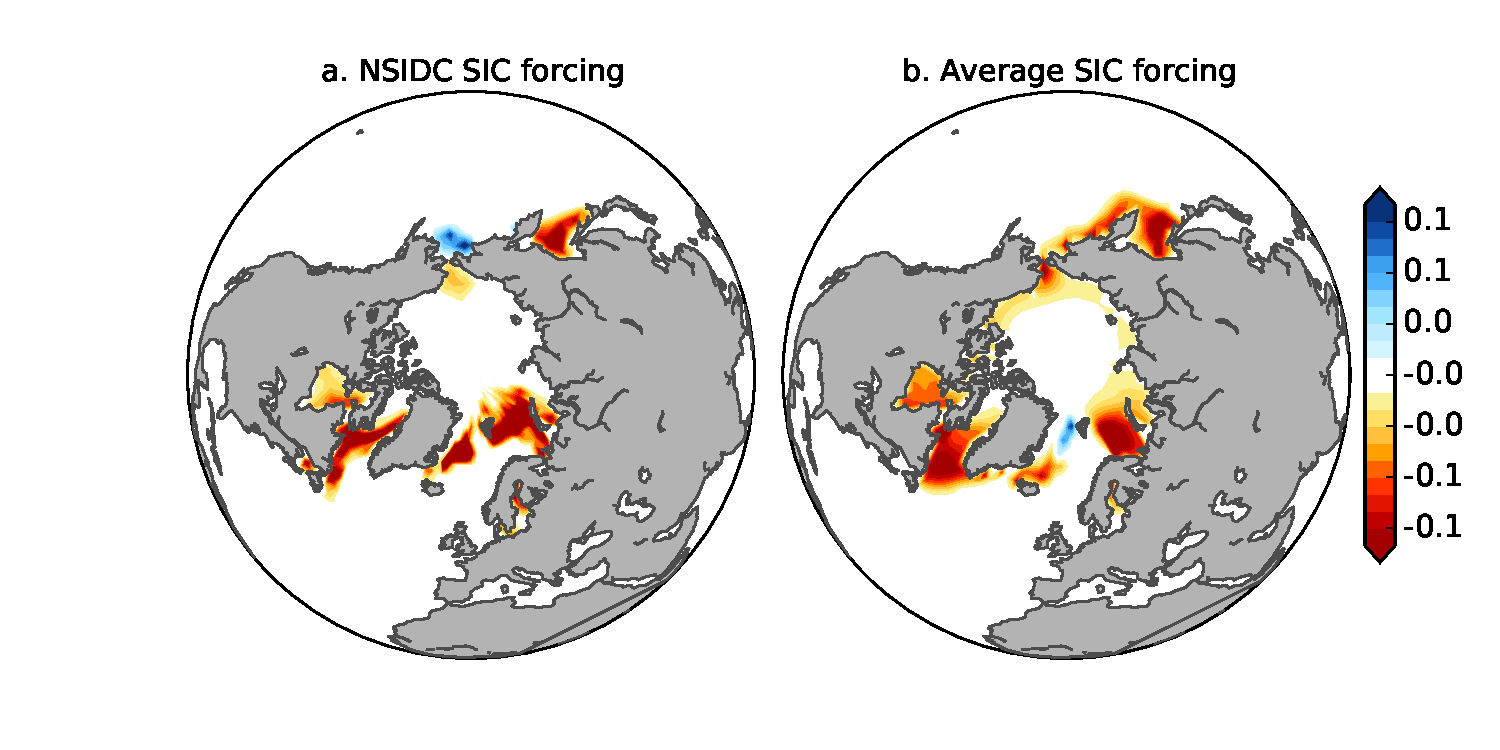
\includegraphics[width=30pc]{SuppFigure1.pdf}
\caption{\textbf{Supplementary Figure 1. Maps of SIC forcing in winter.} a.) Winter sea ice concentration (fraction) boundary forcing for the NSIDC simulations, derived from the NSIDC bootstrap dataset. Anomalies are (2002-11) minus (1979-89). b.) is as (a) except for the boundary forcing averaged from the five CanESM2 historical ensemble members. Anomalies are (2002-12) minus (1979-89).
}
\label{fig:supp1} 
\end{figure}


%\begin{figure}%[htbp] % the star afterwards makes it a one column fig in a 2-col document
%\centering
%\noindent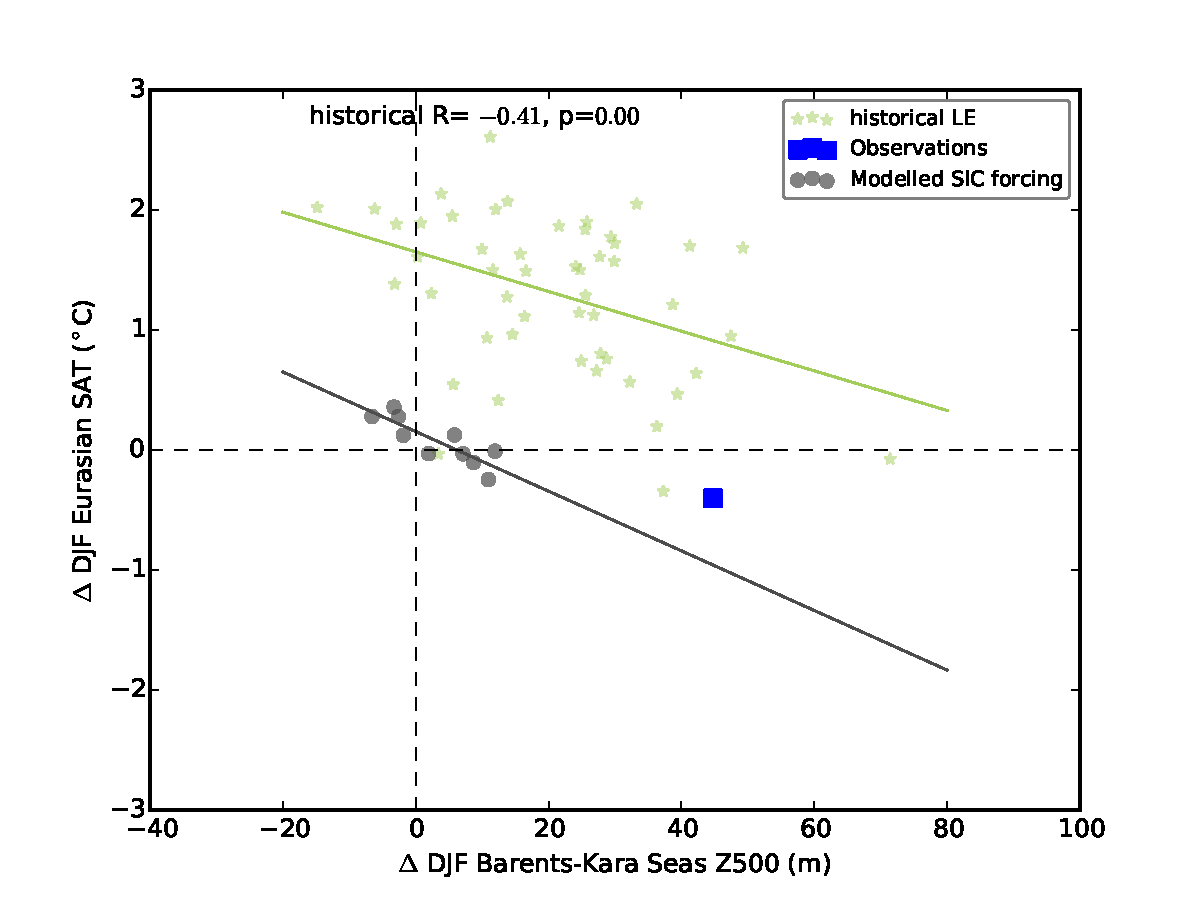
\includegraphics[width=25pc]{SuppFigure2_simsadded.pdf}
%\caption{\textbf{Supplementary Figure 2. CanESM2 large ensemble and observed winter Eurasian SAT and BKS Z500 anomalies.} Historical LE gives a regression slope of -0.17$^\circ$C/10 m, $p$ = 0.003. Simulated 120-year averages are as Figure 5 in main text and give a regression slope of -0.25$^\circ$C/10 m, $p$ = 0.002.
%}
%\label{fig:supp2} 
%\end{figure}
% % FOR Z500 vs Eurasian SAT
% -------- LENat slope, rval, pval: -0.0191453043517 -0.517080959729 0.000120620535074
% -------- LE slope, rval, pval: -0.0165286796574 -0.413836962376 0.00281317881451
% -------- SIMS slope, rval, pval: -0.0248522162816 -0.846875216236 0.00199086631714


\begin{figure}%[htbp] % the star afterwards makes it a one column fig in a 2-col document
\centering
\noindent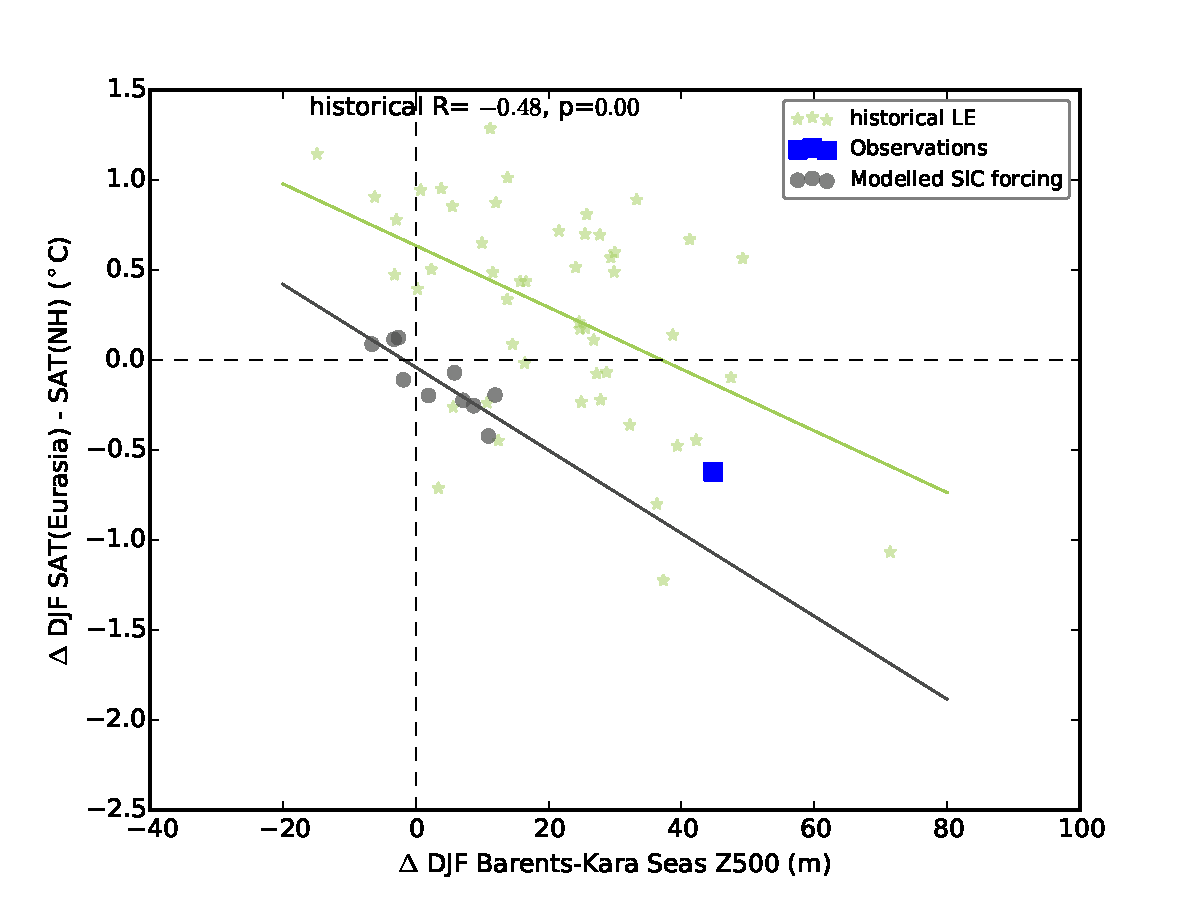
\includegraphics[width=25pc]{SuppFigure2_nhremoved_simsadded.pdf}
\caption{\textbf{Supplementary Figure 2. CanESM2 Historical Large Ensemble winter Eurasian-NH SAT and BKS Z500 anomalies.} Eurasian SAT has northern hemisphere temperature removed, to normalize against the warm bias in the CanESM2 large ensemble. Historical LE gives a regression slope of -0.17$^\circ$C/10 m, $p <$ 0.001. Simulated 120-year averages give a regression slope of -0.23$^\circ$C/10 m, $p$ = 0.002.
}
\label{fig:supp2b} 
\end{figure}
% % FOR Z500 vs Eurasian SAT - NH SAT
% -------- LENat slope, rval, pval: -0.0197128206884 -0.59198196108 5.95247762651e-06
% -------- LE slope, rval, pval: -0.0171532999171 -0.483943293482 0.000369911726737
% -------- SIMS slope, rval, pval: -0.0230542520751 -0.839763760963 0.00236577158697


%% Put the bibliography here, most people will use BiBTeX in
%% which case the environment below should be replaced with
%% the \bibliography{} command.

%\begin{thebibliography}{1}
%\end{thebibliography}
\newpage

%\bibliographystyle{ametsoc}
\bibliography{allrefs}





% ~/bibtexrefs/allrefs  == this is version controlled now, but will have to just copy into current dir?


%% Here is the endmatter stuff: Supplementary Info, etc.
%% Use \item's to separate, default label is "Acknowledgements"

\begin{addendum}
\item[Acknowledgements] 
\item[Author Contributions] 
 \item[Competing Interests] The authors declare that they have no competing financial interests.
\item[Correspondence] Correspondence and requests for materials should be addressed to K.E.M.~(email: kemccusk@uvic.ca).
\end{addendum}

%%
%% TABLES
%%
%% If there are any tables, put them here.
%%

\end{document}
